\section{Interface PINN as an Advanced Method}
\label{sec:interface_pinn}

\subsection{A neural representation of the same interface problem}
We additionally solve the layered problem of Section~2.3 using an
interface-aware physics-informed neural network (PINN). PINNs approximate
the solution by a trainable function constrained by the governing equation
and boundary data \cite{raissi2019pinn}. Here two independent subnetworks
represent the left and right materials. They train jointly through the PDE
residual, the prescribed outer-boundary temperatures, and continuity of
temperature and normal physical flux at $x=1/2$. Prediction selects the
subnetwork by spatial position; there is no output-averaging layer.

Each network has three hidden layers of 64 units with tanh activation. The
combined model has 17,154 parameters. The interface decomposition is related
to the I-PINNs literature \cite{sarma2024interface}, but the present
independent tanh networks differ from the published shared-parameter
architecture. We therefore describe this implementation as an interface
PINN baseline rather than an exact reproduction.

\begin{figure}[H]
\centering
\begin{tikzpicture}[>=Latex,font=\small,
 net/.style={draw,rounded corners=2pt,minimum width=4.3cm,minimum height=1.1cm,align=center},
 objective/.style={draw,rounded corners=2pt,minimum width=7cm,minimum height=1.1cm,align=center}]
 \node[net,draw=teal!70!black,fill=teal!6] (left) at (-3.15,0)
 {\textbf{Left subnetwork}\\Coordinates with $x<1/2$; $a=1$};
 \node[net,draw=violet!70!black,fill=violet!6] (right) at (3.15,0)
 {\textbf{Right subnetwork}\\Coordinates with $x>1/2$; $a=c$};
 \node[objective,draw=orange!80!black,fill=orange!6] (joint) at (0,-2)
 {\textbf{One joint training objective}\\PDE, outer boundary and interface continuity checks};
 \draw[->,thick,teal!70!black] (left.south) -- (left.south|-joint.north);
 \draw[->,thick,violet!70!black] (right.south) -- (right.south|-joint.north);
 \draw[->,dashed,teal!70!black] (joint.west) -- ++(-2,0) |- (left.west);
 \draw[->,dashed,violet!70!black] (joint.east) -- ++(2,0) |- (right.east);
 \node[align=center,font=\footnotesize] at (0,-3)
 {Solid arrows: evaluate constraints. Dashed arrows: update both networks.};
\end{tikzpicture}
\caption{Interface PINN architecture. The two networks train together, and
both are evaluated at interface points. Continuity is a soft constraint,
so its remaining error requires independent checking.}
\label{fig:pinn_architecture}
\end{figure}

\subsection{Training setup and archived optimisation history}
The material contrast is $c=10$, the source is zero, and all four outer
edges use the same exact Dirichlet trace as the preceding layered tests.
Table~\ref{tab:pinn_setup} records the archived training setup. Adam uses
fresh collocation samples at each step; L-BFGS uses a new fixed set.

\begin{table}[H]\centering\small
\caption{Interface PINN configuration from the archived run files.}
\label{tab:pinn_setup}
\begin{tabular}{@{}ll@{}}\toprule
Item & Setting\\\midrule
Device and arithmetic & NVIDIA A100-PCIE-40GB; float64\\
Architecture & Two MLPs, each $2$--$64$--$64$--$64$--$1$, tanh\\
Optimisation & 10,000 Adam steps, learning rate $10^{-3}$; then L-BFGS\\
L-BFGS budget & \texttt{max\_iter=500}, strong-Wolfe line search\\
Interior points & 2,048 per material subdomain\\
Outer-boundary points & 256 per associated edge\\
Interface points & 512\\
Penalty weights & PDE: 1; boundary, temperature and flux continuity: 10 each\\
Random seeds & 11, 22, 33\\\bottomrule
\end{tabular}
\end{table}

Figure~\ref{fig:pinn_training} shows rapid initial reduction of the recorded
Adam objective, followed by fluctuations under resampling. Table~\ref{tab:pinn_endpoints}
gives the last logged Adam objective and the final L-BFGS objective.
The latter is evaluated on a different, fixed collocation set, so these
endpoints are not a controlled optimiser comparison. Only one final
L-BFGS loss per run was saved; no intermediate L-BFGS trajectory is inferred.
The implemented PDE and flux penalties also include scaling, so a training
loss is not itself a physical solution or flux error.

\begin{figure}[H]\centering
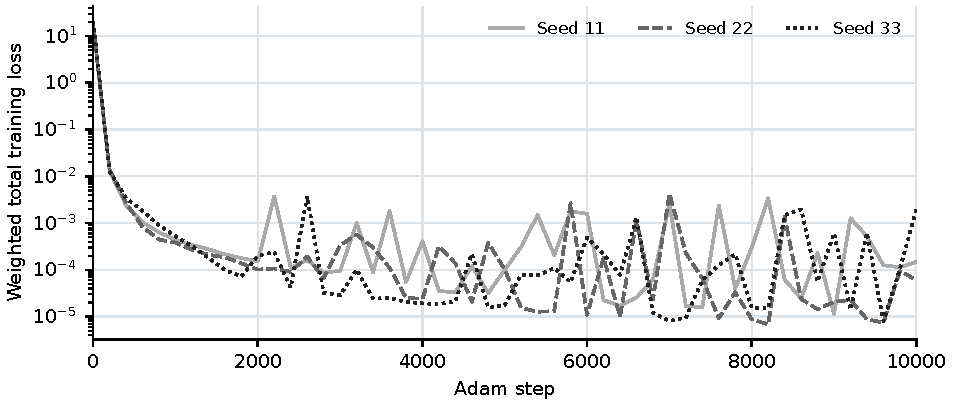
\includegraphics[width=\linewidth]{figures/fig08_pinn_training.pdf}
\caption{Recorded total Adam objective for $c=10$. Logs contain the first
step and then every 200 steps. Fresh samples explain part of the
non-monotone behaviour. Independent physical errors are evaluated separately.}
\label{fig:pinn_training}
\end{figure}

\begin{table}[H]\centering\small
\caption{Archived stage endpoints and synchronised optimisation time.
The L-BFGS column is a final objective, not a full convergence history.}
\label{tab:pinn_endpoints}
\begin{tabular}{@{}rrrrr@{}}\toprule
Seed & Last Adam loss & Final L-BFGS loss & Closure calls & Time (s)\\\midrule
11 & $1.4795\times10^{-4}$ & $3.3990\times10^{-7}$ & 553 & 231.17\\
22 & $6.1087\times10^{-5}$ & $3.4257\times10^{-7}$ & 455 & 226.44\\
33 & $2.0020\times10^{-3}$ & $5.2132\times10^{-7}$ & 570 & 236.22\\\bottomrule
\end{tabular}
\end{table}

The mean training time is $231.3$ seconds, with sample standard deviation
$4.9$ seconds. This covers Adam and L-BFGS optimisation, excluding checkpoint
saving and later evaluation. Closure calls can exceed the maximum L-BFGS
iteration count because line search reevaluates the objective. This is not
a measurement of time to a common target error or of prediction latency.

\subsection{Accuracy compared with harmonic FDM and fitted FEM}
The three methods are evaluated at common points
$(i/63,j/63)$, $i,j=1,\ldots,62$, giving 3,844 interior samples.
Harmonic FDM uses $N=63$ and is evaluated at its nodes; interface-fitted
P1 FEM uses $N=64$ and is evaluated through its actual P1 interpolant.
For the PINN, the same coordinates are passed directly to the trained
networks. We measure sampled relative error
\begin{equation}
 E_{\mathrm{rel,samp}}
 =\left(\frac{\sum_k|\widehat u(z_k)-u_*(z_k)|^2}
 {\sum_k|u_*(z_k)|^2}\right)^{1/2}.
 \label{eq:pinn_sampled_error}
\end{equation}
This is a sampled relative norm, distinct from the continuous reconstructed
$L^2$ norm reported earlier. It also differs from the archive's original
$201\times201$ trapezoidal evaluation. Values must therefore be compared
within the stated protocol rather than substituted across tables.

Flux errors use 62 interface points, $x=1/2$, $y=j/63$,
$j=1,\ldots,62$, with common $+x$ orientation and exact flux $-20/11$.
We use the shared crossing-face flux for FDM and both one-sided traces for
FEM and PINN, taking the maximum absolute error. For each PINN seed the
metrics are computed first, then averaged across seeds; predictions are
not averaged before measuring error.

\begin{figure}[H]\centering
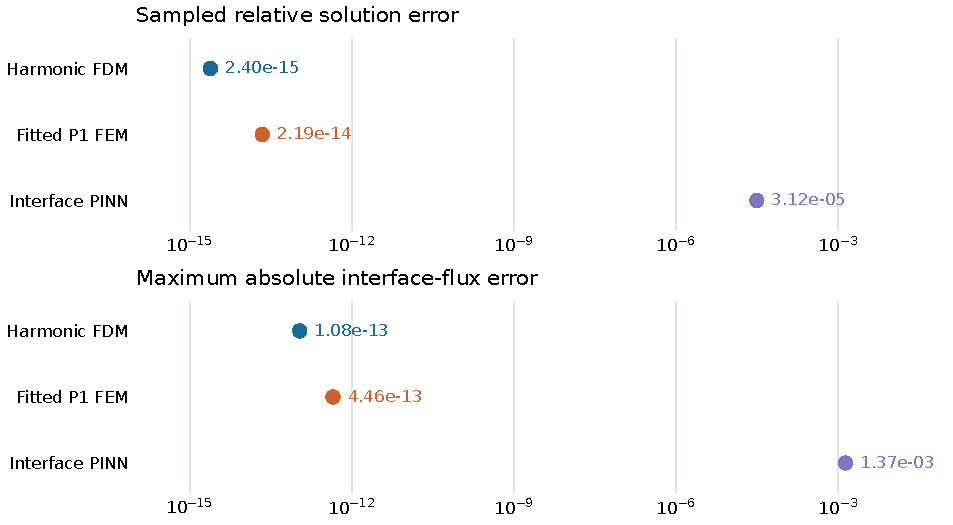
\includegraphics[width=\linewidth]{figures/fig09_pinn_accuracy.pdf}
\caption{Common-sample comparison on the layered $c=10$ benchmark.
Smaller errors lie to the left. The PINN marker is the mean of three
seed-specific errors. Classical errors are near numerical precision for
this specially representable solution; their last digits do not establish
a meaningful accuracy ranking.}
\label{fig:pinn_accuracy}
\end{figure}

\begin{table}[H]\centering\small
\caption{Common-sample accuracy. Different FDM/FEM mesh parities are
intentional, so this is not an equal-degree-of-freedom comparison.}
\label{tab:pinn_accuracy}
\begin{tabular}{@{}lrr@{}}\toprule
Method & $E_{\mathrm{rel,samp}}$ & Max. absolute interface-flux error\\\midrule
Harmonic FDM, $N=63$ & $<10^{-12}$ & $<10^{-12}$\\
Fitted P1 FEM, $N=64$ & $<10^{-12}$ & $<10^{-12}$\\
Interface PINN, three-seed mean & $3.12\times10^{-5}$ & $1.37\times10^{-3}$\\\bottomrule
\end{tabular}
\end{table}

The classical methods reproduce the layered solution to approximately
numerical precision because it is piecewise linear: harmonic FDM recovers
the exact nodal values and the fitted P1 space contains the exact solution.
The PINN approximates the same solution but retains larger solution and
flux errors. The result demonstrates an alternative interface formulation,
not an accuracy advantage on this benchmark. Its GPU training time also
cannot be directly ranked against the earlier CPU timings for a different
smooth problem and mesh.

\paragraph{Single-network ablation.}
As a secondary check, we replay three archived single-network PINN runs
at the same common points, using seeds 11, 22 and 33 and the same configured
Adam/L-BFGS budgets. The width and depth of each network and the collocation
counts and penalty weights are unchanged. Table~\ref{tab:pinn_ablation}
compares the mean seed-specific errors. A single smooth tanh network has
one derivative at the interface and cannot represent an exact derivative
jump while keeping a nonzero continuous physical flux when $a_L\ne a_R$.
Two subnetworks can represent different one-sided derivatives.

\begin{table}[H]\centering\small
\caption{Archived architectural ablation, $c=10$, same common-sample norms
as Table~\ref{tab:pinn_accuracy}. The interface model has twice as many
parameters, so this is not a parameter-matched isolation of decomposition.}
\label{tab:pinn_ablation}
\begin{tabular}{@{}lrrr@{}}\toprule
Representation & Parameters & $E_{\mathrm{rel,samp}}$ & Max. flux error\\\midrule
Single PINN & 8,577 & $3.10\times10^{-1}$ & $2.81$\\
Interface PINN & 17,154 & $3.12\times10^{-5}$ & $1.37\times10^{-3}$\\\bottomrule
\end{tabular}
\end{table}

These runs support the interface representation on this benchmark, but do
not establish general superiority or isolate the effect of parameter count.
Both architectures use soft boundary and flux constraints. This ablation
supplements the main FDM/FEM comparison and does not replace it.

\subsection{Reproduction and limitations}
Checkpoints, logs, configuration, device metadata and matching model code
are retained under \path{support/interface_pinn/}.
The script \path{support/interface_pinn/reevaluate.py} replays all six
checkpoints and solves the classical references on CPU without retraining;
plotting code and source hashes accompany it. Paths in this section are
relative to \path{project2/report/} in the repository. No error-versus-step or
per-step timing history was archived. Soft constraints do not guarantee
continuity between samples. Curved interfaces and comparisons at equal
accuracy and compute require further experiments.
